In the course of all the described experiments, the performance of both the simple and the attentive Texter were steadily improved. What was missing was the hoped-for increase in performance of the attentive Texter compared to the simple version. Instead, the simple Texter actually performs better on many text sets. In order to get to the bottom of the cause, the attention mechanism should be investigated to find out whether the basic assumption that the class embeddings react to sentences in which class-typical keywords appear can be verified. In particular, it was examined (1) whether the trained class embeddings match keywords that are typical for the respective class, (2) whether the attention block favors sentences that would yield clear classification results on their own, and (3) how the attention values relate to the sentence embeddings on the word level.

Regarding the first question, the assumption was that the class embeddings converge against keywords that are particularly meaningful for a class during training. To confirm this assumption, the class embeddings $class_c$, of a trained texter were matched, i.e. scalar multiplied, with all word embeddings $word_w$ of the vocabulary. The resulting similarity values $\langle class_c, word_w \rangle$ were sorted, and the values with the largest absolute values $|\langle class_c, word_w \rangle|$ were examined for plausibility. Thereby, the indices $1 <= c <= |C|$ and $1 <= w <= |V|$ specify one of the classes from the class set $C$ and a word from the vocabulary $V$, respectively. It was expected that the words that lead to large, positive similarities would be keywords in favor of the regarded class, while words that lead to high negative similarities in terms of amount would speak against the class. As an example, the embedding of the word ``American'' was expected to be similar to the class embedding of $(x, from, USA)$ -- in contrast to the embedding of ``French''. Table \autoref{tab:5_experiments/3_texter/2_static/9_attention/top_words} shows the top words with the highest positive similarities the attentive Texter reacts to after being trained on the CDE split with cde-irt-5-clean texts.

\begin{table}[h]
    \makebox[\textwidth][c]{
        \begin{tabular}{ l l }
    \toprule

    \multicolumn{1}{l}{\textbf{Class}} &
    \multicolumn{1}{l}{\textbf{Top matching words}} \\

    \midrule

    $(x, from, USA)$ & nhs, mid-engined, ruislip, filipina   \\
    $(x, is, writer)$                               & recepter, 1/4, makovsky, pairwise     \\
    $(x, speaks, English)$    & republish, in-demand, brahmos, steyr \\

    \bottomrule
\end{tabular}

    }
    \caption{Top words matching the class embeddings of the static, attentive Texter. The words do not resemble the classes.}
    \label{tab:5_experiments/3_texter/2_static/9_attention/top_words}
\end{table}

Contrary to expectations, the top words do not clearly relate to the respective classes. With a few exceptions such as ``Maryland'' and ``BBC'', which occur further down in the suggestions for $(x, from, USA)$ or $(x, speaks, English)$, the words appear rather random. Given the infrequent occurrence of top words, overfitting seemed like a reasonable explanation. However, the top words change with repeated training runs, so it appears more likely that the word embeddings simply happened to be close to the learned class embeddings. However, if this affects only a small proportion of top words and the class embeddings are mostly close to relevant words, this should have little impact on the generalizability of the model. Whether this relation also applies to more frequent keywords has been investigated in the third experiment.

Beforehand, the second question, asking whether the attention mechanism weights the sentences most heavily that are also the most meaningful on their own, has been answered. For this purpose, the attentive Texter has been extended by a method that bypasses the attention mechanism during inference. The trained model is still passed multiple sentences per entity when called, but instead of these being used to calculate entity embeddings in the attention block, the sentence embeddings are pushed directly through the classification block. In the following, that modified version of the Texter, which yields the class logits for each individual sentence, is denoted as the function $\psi$. However, since the linear layers of the complex model were actually trained on the entity embeddings, this experiment only works with a Texter whose attention block uses the softmax function because the sigmoid version, does not guarantee that the individual sentence embeddings have the same order of magnitude as the entity embeddings.

\autoref{tab:5_experiments/3_texter/2_static/9_attention/kari_soft} presents exemplary results for the entity ``Kari Hotakainen'', a Finnish writer. At the edges, the table shows the four most frequent classes in the CDE split, the example entity's five sentences, the class logits predicted by the Texter as well as the respective ground truth values. The table's main block shows the attention value for each class-sentence combination in addition to the class logit produced by the $\psi$ function, i.e. the class prediction that would be obtained when bypassing the attention mechanism. The entity ``Kari Hotakainen'' has been chosen because its quantitative results are close to the average metric values for the cde-irt-5-clean text set: Considering only the selected classes, the predictions result in a precision of 33\%, a recall of 100\%, and thus an overall F1 score of 33\%, which is close to the Texter dataset's 37.6\%. In addition, the short sentences are well suited for presentation.

\begin{table}[t]
    \makebox[\textwidth][c]{
        \begin{tabular}{|l|l|r|r|r|r|}
\hline
\multicolumn{1}{|c|}{\multirow{2}{*}{\textbf{Sentence}}} &
   &
  \multicolumn{4}{c|}{\textbf{Class}} \\ \cline{2-6} 
\multicolumn{1}{|c|}{} &
   &
  \multicolumn{1}{c|}{\textbf{\begin{tabular}[c]{@{}c@{}}from\\ USA\end{tabular}}} &
  \multicolumn{1}{c|}{\textbf{\begin{tabular}[c]{@{}c@{}}is\\ writer\end{tabular}}} &
  \multicolumn{1}{c|}{\textbf{\begin{tabular}[c]{@{}c@{}}speaks\\ English\end{tabular}}} &
  \multicolumn{1}{c|}{\textbf{\begin{tabular}[c]{@{}c@{}}is\\ actor\end{tabular}}} \\ \cline{2-6} 
 &
  $\phi_c(S)$ &
  -1.26 &
  1.98 &
  0.22 &
  0.55 \\ \cline{2-6} 
 &
  GT &
  \multicolumn{1}{c|}{0} &
  \multicolumn{1}{c|}{1} &
  \multicolumn{1}{c|}{0} &
  \multicolumn{1}{c|}{0} \\ \hline
\begin{tabular}[c]{@{}l@{}}the film was written by\\ kari \_ and juha \_\end{tabular} &
  \multirow{5}{*}{\begin{tabular}[c]{@{}l@{}} \\ \\ \\ \\ $\sigma(\langle e_c, e_s \rangle)$ \\ $\psi_c(s)$\end{tabular}} &
  \begin{tabular}[c]{@{}r@{}} 0.16 \\ -0.16 \end{tabular} &
  \begin{tabular}[c]{@{}r@{}} 0.11 \\  2.01 \end{tabular} &
  \begin{tabular}[c]{@{}r@{}} 0.12 \\  0.88 \end{tabular} &
  \begin{tabular}[c]{@{}r@{}} 0.13 \\  0.11 \end{tabular} \\ \cline{1-1} \cline{3-6} 
\begin{tabular}[c]{@{}l@{}}it is based on kari \_ semi-\\ autobiographical novel \_\end{tabular} &
   &
  \begin{tabular}[c]{@{}r@{}} 0.22 \\ -1.06 \end{tabular} &
  \begin{tabular}[c]{@{}r@{}} \textbf{0.27} \\  \textbf{2.69} \end{tabular} &
  \begin{tabular}[c]{@{}r@{}} 0.21 \\  0.57 \end{tabular} &
  \begin{tabular}[c]{@{}r@{}} 0.22 \\ -0.06 \end{tabular} \\ \cline{1-1} \cline{3-6} 
\begin{tabular}[c]{@{}l@{}}the film is inspired by kari \\ \_ novel of the same name.\end{tabular} &
   &
  \begin{tabular}[c]{@{}r@{}} 0.12 \\  0.16 \end{tabular} &
  \begin{tabular}[c]{@{}r@{}} 0.26 \\  2.40 \end{tabular} &
  \begin{tabular}[c]{@{}r@{}} 0.17 \\  \textbf{1.24} \end{tabular} &
  \begin{tabular}[c]{@{}r@{}} 0.11 \\  0.02 \end{tabular} \\ \cline{1-1} \cline{3-6} 
\begin{tabular}[c]{@{}l@{}}the unknown \_ \_ () is an\\ authorised biography on \\ finnish racing driver \_ \_ \\ by kari \_\end{tabular} &
   &
  \begin{tabular}[c]{@{}r@{}} \textbf{0.32} \\ \textbf{-2.87} \end{tabular} &
  \begin{tabular}[c]{@{}r@{}} 0.23 \\  1.04 \end{tabular} &
  \begin{tabular}[c]{@{}r@{}} \textbf{0.29} \\ -0.64 \end{tabular} &
  \begin{tabular}[c]{@{}r@{}} 0.26 \\  1.01 \end{tabular} \\ \cline{1-1} \cline{3-6} 
\begin{tabular}[c]{@{}l@{}}\_ is a 2002 novel by \\ finnish author kari \_\end{tabular} &
   &
  \begin{tabular}[c]{@{}r@{}} 0.18 \\ -0.57 \end{tabular} &
  \begin{tabular}[c]{@{}r@{}} 0.13 \\  1.24 \end{tabular} &
  \begin{tabular}[c]{@{}r@{}} 0.22 \\ -0.07 \end{tabular} &
  \begin{tabular}[c]{@{}r@{}} \textbf{0.28} \\  \textbf{1.03} \end{tabular} \\ \hline
\end{tabular}

    }
    \caption{Predicting facts for the example entity Kari Hotakainen using the static, attentive Texter with the \textbf{softmax} function in the attention block. For an entity with a sentence set $S$, $\phi_c(S)$ and GT give the predicted class logits and ground truth. For each class $c$ and sentence $s$, $A_{cs}$ gives the class-sentence attention. $\psi_c(s)$ yields a sentence's individual class logits if the attention mechanism is skipped. The largest values in terms of amount are marked bold for each class (column-wise). The model prefers sentences that would come to a strong decision by themselves.}
    \label{tab:5_experiments/3_texter/2_static/9_attention/kari_soft}
\end{table}

\autoref{tab:5_experiments/3_texter/2_static/9_attention/kari_soft} shows that, for the example entity, the attentive Texter does indeed prefer those sentences that would give a clear result on their own for three of the four classes. In the fourth case, the model heavily incorporates a sentence that has a rather uncertain outcome. Despite that the respective prediction would have been correct on its own, the model should not have focused on it. Looking at other sentences that have been focused, further misjudgments become apparent, such as the cases where the texter relied on the fifth and second sentences to predict the classes $(x, speaks, English)$ and $(x, is, actor)$, respectively, which both lead to unreliable decisions on their own. Overall, however, it is noticeable that meaningful sentences are more strongly included in the entity embeddings.

Still, the effective focus on sentences that would lead to clear predictions on their own is of no use if the sentence's prediction is wrong. For example, in \autoref{tab:5_experiments/3_texter/2_static/9_attention/kari_soft}, the first three sentences incorrectly indicate that Kari Hotakainen speaks English. Also, he is predicted to be an actor which is not the case -- that prediction is probably made due to the $(x, is, actor)$ class's general high posterior probability as the dataset contains many actors. At least, however, the Texter was less certain about its false predictions than it was about the true ones.

What is still missing, however, is a clear prioritization of the sentences. For example, as a human, one would give the last sentence a much higher weighting when it comes to the negation of the class $(x, from, USA)$ due to the fragment ``by finnish author kari hotakainen''. The problem is that using static word embeddings, the model cannot recognize at this point that the word ``finnish'' is much more relevant than in the preceding sentence in which the same word does not refer to the entity itself. Another problem is that repeating the experiment often leads to different sentence prioritizations. Although the entity's class logits, and thereby the overall class predictions, change only slightly between experiments, this observation questions the attention mechanism's ability to explain its text-based decision reliably.

This uncertainty about the order of the sentences also exists in the final model that uses the sigmoid function, although to a lesser extent. Analogous to \autoref{tab:5_experiments/3_texter/2_static/9_attention/kari_soft},  \autoref{tab:5_experiments/3_texter/2_static/9_attention/kari} shows the attention values after the sigmoid function has been applied instead of the softmax, which is why the probabilities no longer sum up to 100\% column-wise. Furthermore, \autoref{tab:5_experiments/3_texter/2_static/9_attention/kari_soft} misses the results of the $\psi$ function which cannot be calculated here as explained before. The shown figures imply that the sigmoid version achieves a higher overall precision due to the correct prediction of $(x, is, actor)$ and that the inclusion of uncertain sentences is generally lower. But still, the order between the relevant sentences varies among training runs.

\begin{table}[t]
    \makebox[\textwidth][c]{
        \begin{tabular}{| l | l | r r r r |}
\hline
\multicolumn{1}{|c|}{\multirow{2}{*}{\textbf{Sentence}}} &
   &
  \multicolumn{4}{c|}{\textbf{Class}} \\ \cline{3-6}
\multicolumn{1}{|c|}{} &
   &
  \multicolumn{1}{c}{\textbf{\begin{tabular}[c]{@{}c@{}}from\\ USA\end{tabular}}} &
  \multicolumn{1}{c}{\textbf{\begin{tabular}[c]{@{}c@{}}is\\ writer\end{tabular}}} &
  \multicolumn{1}{c}{\textbf{\begin{tabular}[c]{@{}c@{}}speaks\\ English\end{tabular}}} &
  \multicolumn{1}{c|}{\textbf{\begin{tabular}[c]{@{}c@{}}is\\ actor\end{tabular}}} \\ \cline{2-6}
 &
  \multicolumn{1}{c|}{$\phi_c(S)$} &
  -1.43 &
  2.19 &
  0.85 &
  -0.14 \\
 &
  \multicolumn{1}{c|}{GT} &
  \multicolumn{1}{r}{0} &
  \multicolumn{1}{r}{1} &
  \multicolumn{1}{r}{0} &
  \multicolumn{1}{c|}{0} \\ \hline
\begin{tabular}[c]{@{}l@{}}the film was written by\\ kari \_ and juha \_\end{tabular} &
  \multirow{5}{*}{\begin{tabular}[c]{@{}l@{}} \\ \\ \\ \\ $\sigma(\langle e_c, e_s \rangle)$ \end{tabular}} &
  0.47 &
  \textbf{0.74} &
  0.27 &
  0.36 \\ \cline{1-1} \cline{3-6} 
\begin{tabular}[c]{@{}l@{}}it is based on kari \_ semi-\\ autobiographical novel \_\end{tabular} &
   &
  0.40 &
  0.54 &
  0.23 &
  0.23 \\ \cline{1-1} \cline{3-6} 
\begin{tabular}[c]{@{}l@{}}the film is inspired by kari \\ \_ novel of the same name.\end{tabular} &
   &
  0.36 &
  0.45 &
  \textbf{0.13} &
  \textbf{0.21} \\ \cline{1-1} \cline{3-6} 
\begin{tabular}[c]{@{}l@{}}the unknown \_ \_ () is an\\ authorised biography on \\ finnish racing driver \_ \_ \\ by kari \_\end{tabular} &
   &
  0.31 &
  0.62 &
  0.20 &
  0.30 \\ \cline{1-1} \cline{3-6} 
\begin{tabular}[c]{@{}l@{}}\_ is a 2002 novel by \\ finnish author kari \_\end{tabular} &
   &
  \textbf{0.27} &
  0.57 &
  0.27 &
  0.38 \\ \hline
\end{tabular}

    }
    \caption{Predicting facts for the example entity Kari Hotakainen using the static, attentive Texter with the \textbf{sigmoid} function in the attention block. For an entity with a sentence set $S$, $\phi_c(S)$ and GT give the predicted class logits and ground truth. For each class $c$ and sentence $s$, $A_{cs}$ gives the class-sentence attention. The sigmoid values that deviate most from 0.5 are marked bold for each class (column-wise). The model tends to score sentences that favor a class high and unfavorable ones low.}
    \label{tab:5_experiments/3_texter/2_static/9_attention/kari}
\end{table}

Another interesting insight is provided by the third experiment on the attention mechanism, which investigates how attention values derive from word embeddings. A prerequisite for the experiment is the usage of mean pooling, i.e. the calculation of the sentence embeddings as the mean of the respective word embeddings. In this case, the scalar product of a class embedding $\textbf{class}_c$ and a sentence embedding $\textbf{sent}_s$ can be broken down to the mean of the scalar products between the class embedding and the sentence's word embeddings $\textbf{word}_w$ where $1 <= w <= N$ is the word's position within the sentence:

\begin{align}
    \langle \textbf{class}_c, \textbf{sent}_s \rangle
    = \langle \textbf{class}_c, \frac{1}{N} \sum_{w=1}^N \textbf{word}_w \rangle
    = \frac{1}{N} \sum_{w=1}^N \langle \textbf{class}_c, \textbf{word}_w \rangle
    \label{eq:5_experiments/3_texter/2_static/9_attention/word_embs}
\end{align}

Leveraging this relationship, \autoref{fig:5_experiments/3_texter/2_static/9_attention/kari_softmax} illustrates which words influence the overall scalar products between the class and sentence embeddings of the example entity Kari Hotakainen the most. Words that have a similar or opposite embedding to the class embedding are highlighted in yellow and purple, respectively. The expectation was that class-specific keywords would be clearly visible. During the experiment, it was noticed by coincidence that the result for softmax- and sigmoid-based attention mechanisms differ significantly. Therefore, each sentence is shown twice per class -- once for the softmax function and once for sigmoid function.

\begin{figure}
    \centering
    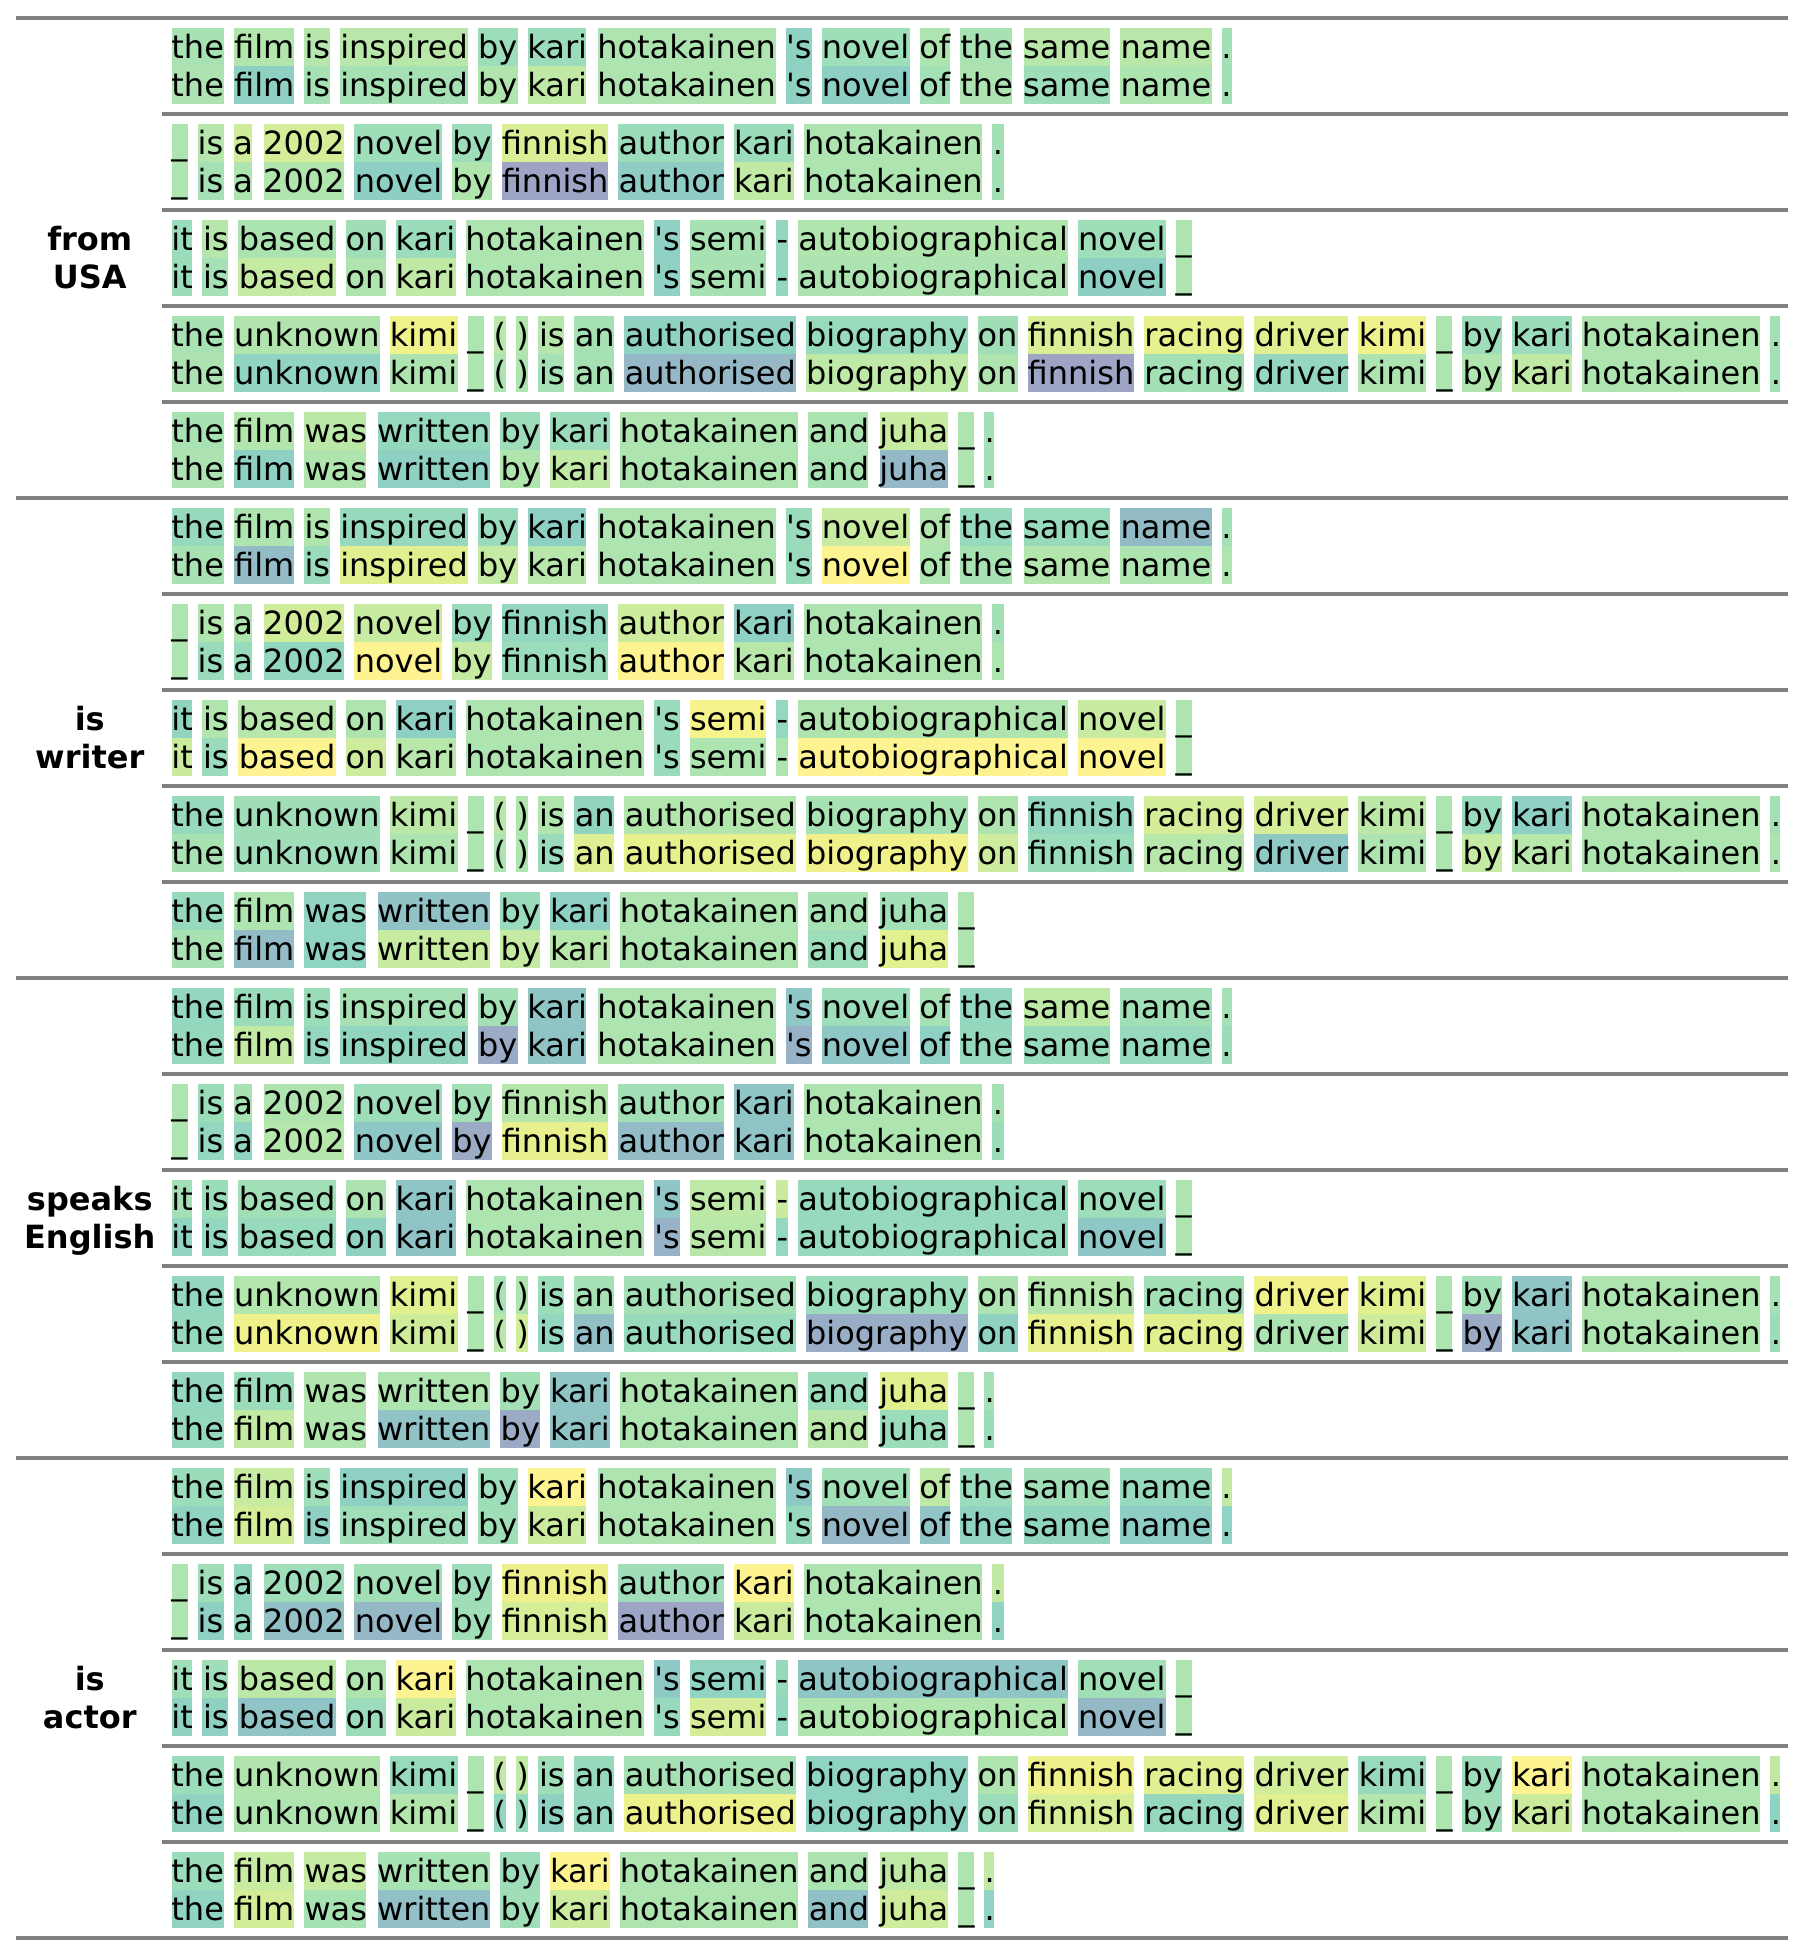
\includegraphics[width=\textwidth]{5_experiments/3_texter/2_static/9_attention/kari_softmax}
    \caption{Illustration of how the attention values for the example entity Kari Hotakainen can be traced back to class-related keywords that influence the overall sentence embeddings. Each cell shows the same sentence from the view of the Texter using either the softmax function (top) or the sigmoid function (bottom) function. High (low) class-word attentions are highlighted in yellow (purple). The Texter that uses the sigmoid function reacts much more to class-related keywords.}
    \label{fig:5_experiments/3_texter/2_static/9_attention/kari_softmax}
\end{figure}

Although the use of the softmax or the sigmoid function in the attention block leads to very similar F1 scores, the training of the word embeddings seems to differ significantly in both cases. When using the sigmoid function, the learned class embeddings attend to class-relevant keywords as expected whereas this is not the case with the softmax function. For example, the sigmoid version learns that the words ``novel,'' ``author,'' and ``biography'' are closely related to the class $(x, is, author)$ and that Finns tend to be likely to speak English. Conversely, ``Finnish'' and the name ``Juha'' speak against an origin from the US, and, apparently, authors are rarely actors at the same time. In contrast, the softmax version attends to the names ``Kimi'' and ``Kari'' whose relationships  to $(x, from, USA)$ and $(x, is, actor)$ are not obvious.

In summary, the assumptions regarding the attention mechanism are only partially supported empirically and no reliable prioritization between an entity's sentences is established, which is probably the reason for the missing performance improvement of the attentive Texter compared to the simple Texter. One possible reason has already been mentioned: With static word embeddings, the model cannot detect whether a potentially class-relevant keyword refers to the entity or not. This becomes even more obvious with a long sentence like the following of which there are many in the IRT text sets:

\begin{displayquote}
    The Chilean writer Ricardo Cuadros said that McOndo irreverence for Latin American literary tradition, its thematic–stylistic concentration upon the pop culture of the United States, and the literatures’ apolitical tone, are dismissive of the literary ideas, writing style, and narrative techniques of the generation of Latin American writers (García Márquez, Vargas Llosa, Carpentier, Fuentes, et al.) who lived under, opposed, and (occasionally) were repressed by dictators.
\end{displayquote}

The sentence is associated with a Latin American writer who was classified as an American due to the keywords ``United'', ``States'' and the twice occurring ``American'' whose relation to ``Latin'' cannot be captured by static word embeddings. When trying to identify the entity in question, a second problem reveals itself concerning long sentences: Even as a human, it is not recognizable that, with all the named entities, the text is about the Peruvian writer Mario Vargas Llosa and not the Chilean Ricardo Cuadros.
